En este capitulo se brinda una explicación de Apolo y sus especificaciones técnicas y como este soporta desde su arquitectura la computación paralela. 

Se brinda también una  descripción de lo que es un grafo y su importancia, para modelarlos se utilizan las librerías paralelas de Boost, por lo que se explica que es Boost, las cuales están escritas en C++ y utilizan MPI como mecanismo de comuniacación.


\section{Apolo}

Apolo es el Centro de Computación Científica de la Universidad EAFIT, el cual tiene por objetivo principal apoyar la investigación y el desarrollo del país y de la región. 

Para cumplir con tal objetivo, presta sus servicios para la investigación, tanto en el mundo académico como en la industria, mediante la simulaciones computacionales en un equipo de altos recursos, utilizando técnicas de computación de alto rendimiento, también conocida como computación paralela.

Apolo se compone de un equipo físico (todos el hardware y la infraestructura necesaria de un clúster para el computo en paralelo) y un equipo humano capacitado tanto para la administración y mantenimiento del software y hardware, como  para la capacitación de nuevos usuarios y el apoyo a los usuarios existentes.

\textbf{Especificaciones Técnicas} 

La infraestructura física de Apolo esta compuesta por:

\begin{itemize}
	\item 40 Servidores de 4 núcleos: Blade HP ProLiant DL140 Generation 3\cite{techDL140}

	\begin{figure}[H]
		\centering
		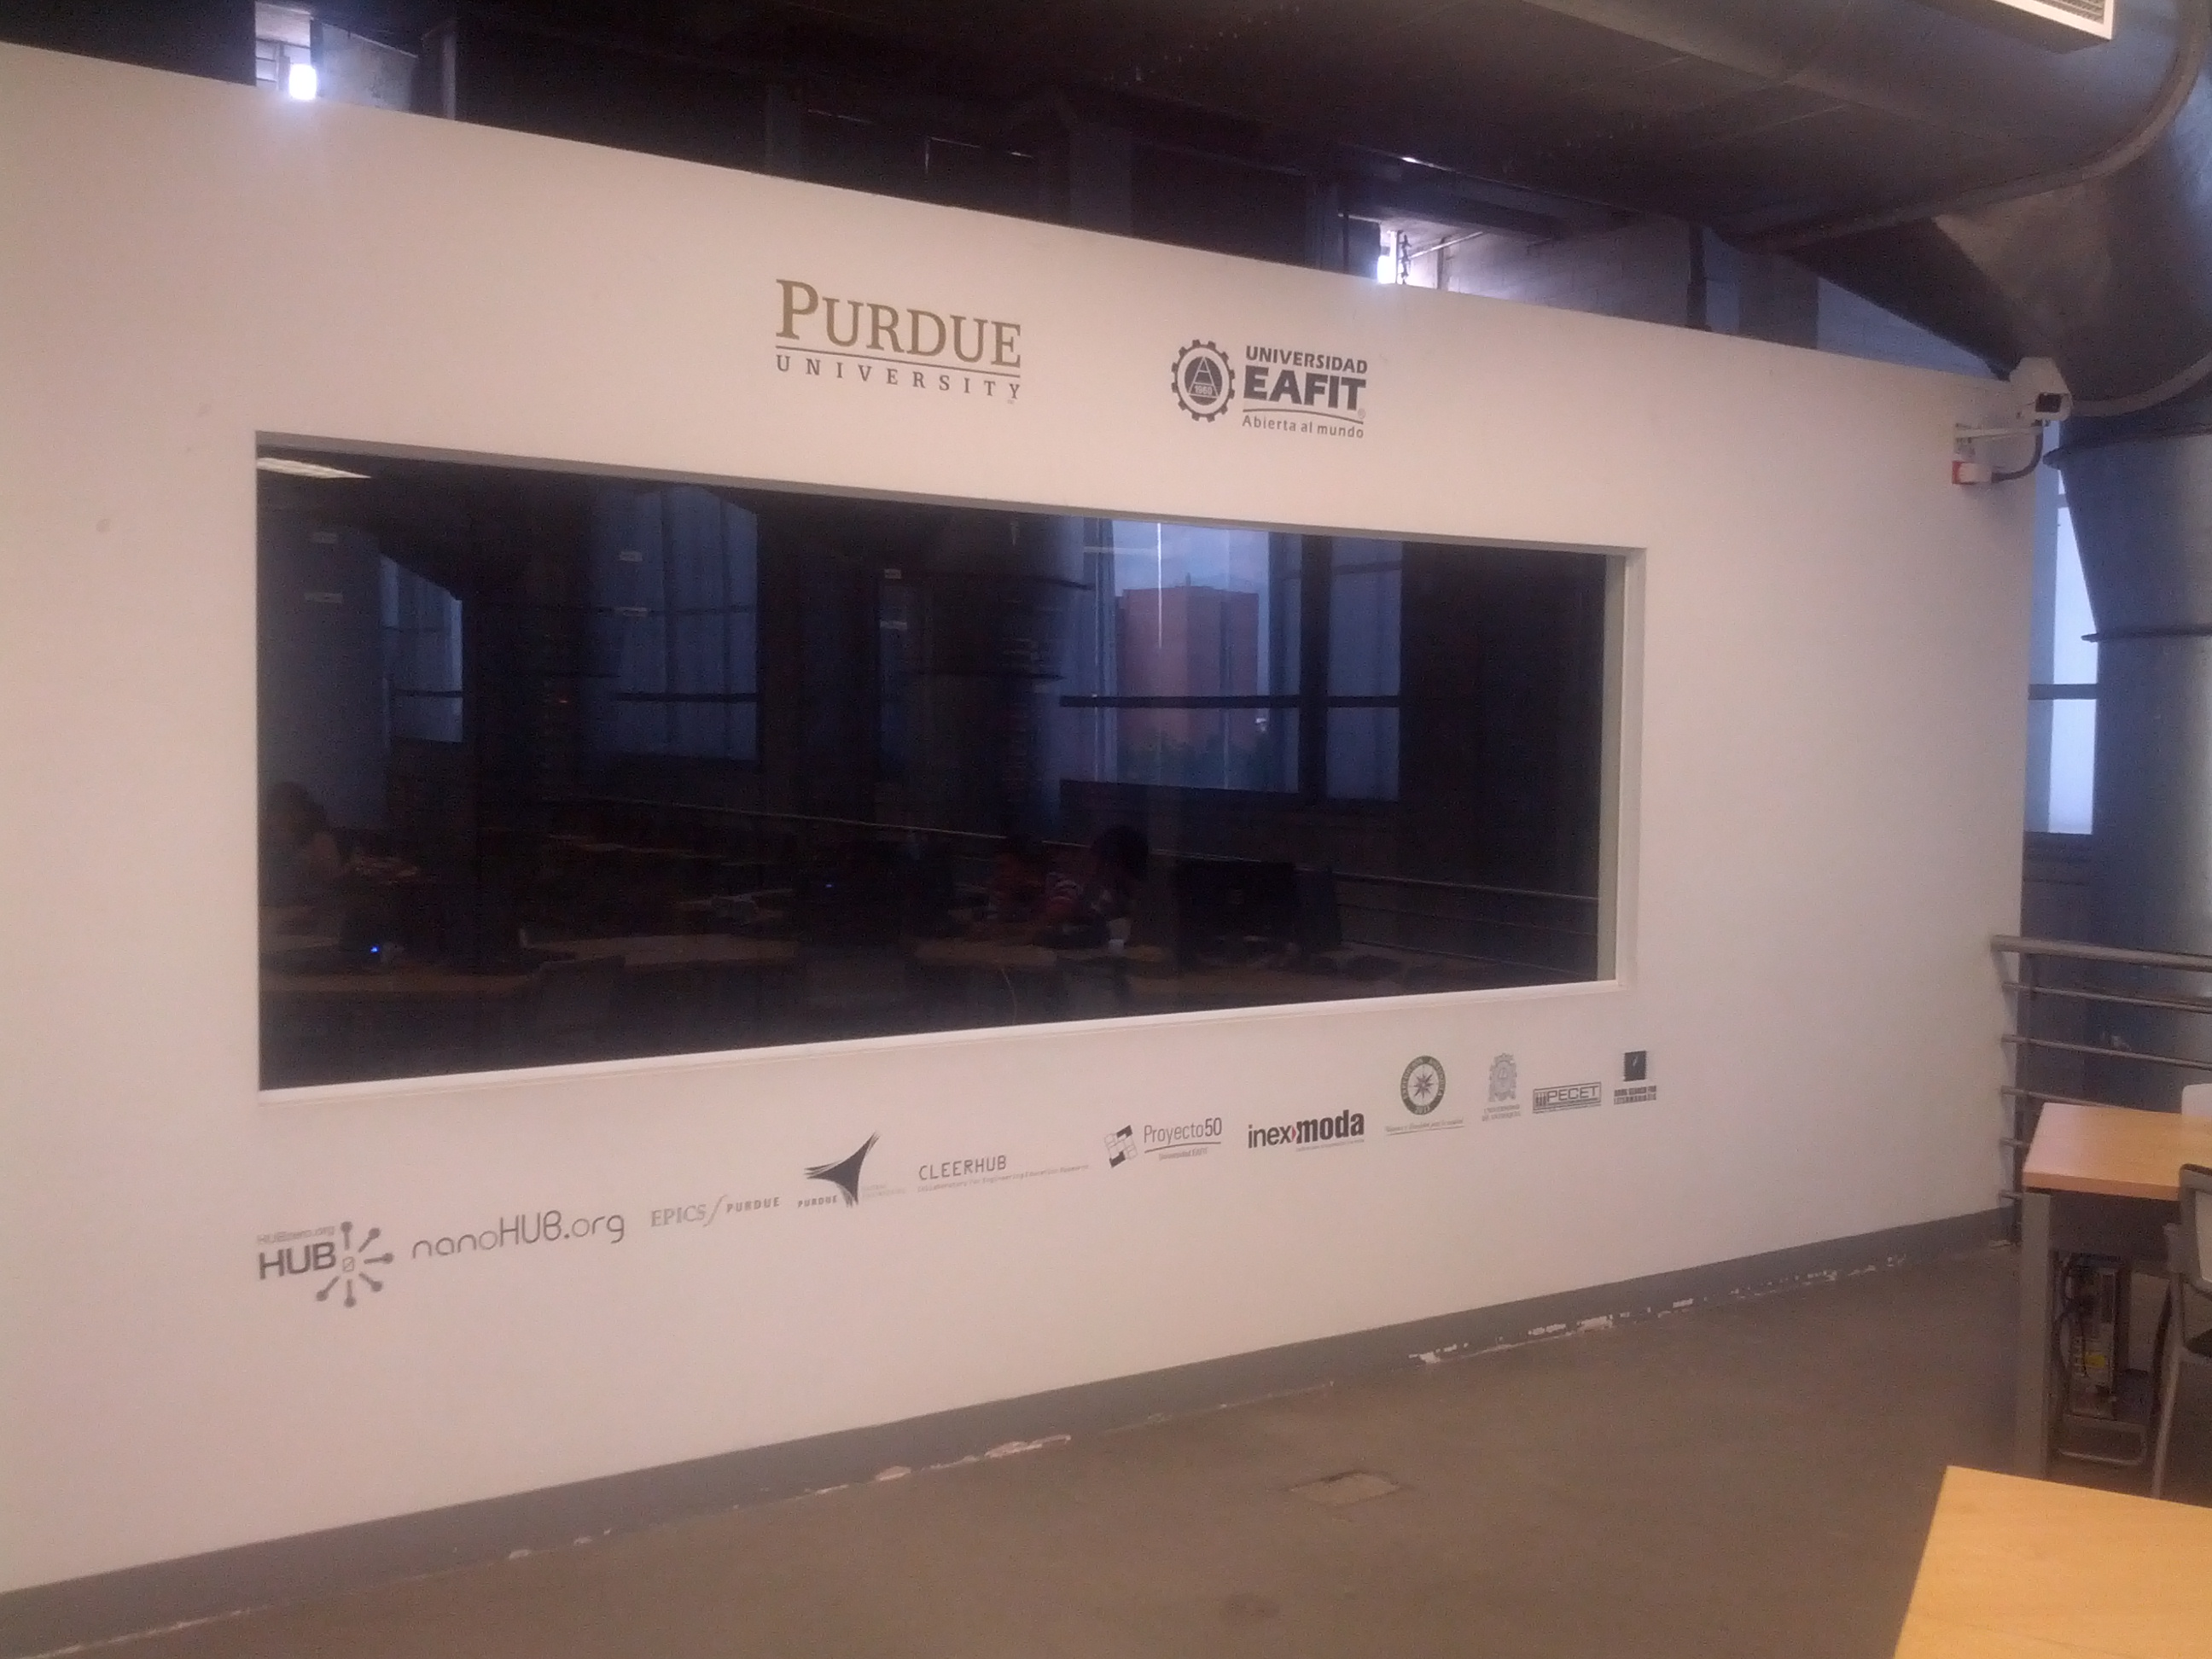
\includegraphics[width=0.5\textwidth]{aux/apolo}
		\caption[Blad HProLiant DL140]{}
		%(tomada de \citP {WikiEmotion)}
		%\label{F-dimensions-emotion}
	\end{figure}
	
 	
	\item  6 servidores de 8 núcleos: Blade HP Proliant BL460c G1\cite{techBL460}


	\begin{figure}[H]
		\centering
		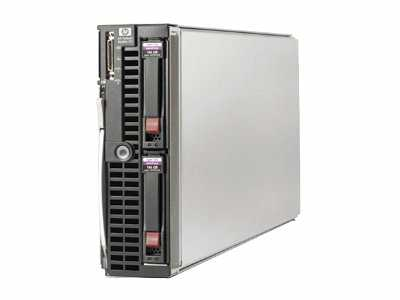
\includegraphics[width=0.5\textwidth]{aux/Aguadas}
		\caption[Blade HP BL460]{}
		%(tomada de \cite{WikiEmotion)}
		%\label{F-dimensions-emotion}
	\end{figure}
	

	\item 40  servidores de 8 núcleos: Blade Dell PowerEdge 1950\cite{teckDell1950}

	\begin{figure}[H]
		\centering
		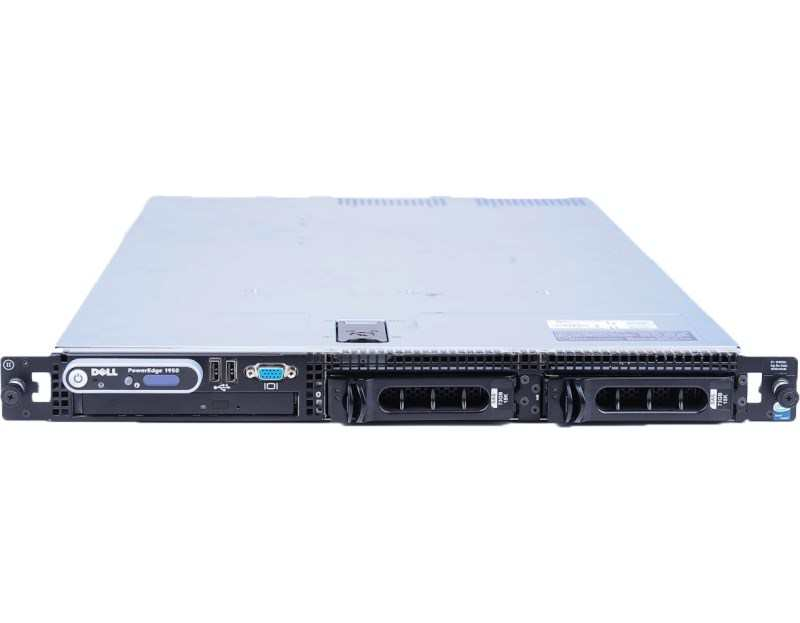
\includegraphics[width=0.5\textwidth]{aux/1950}
		\caption[Blade Dell PowerEdge 1950]{}
		%(tomada de \cite{WikiEmotion)}
		%\label{F-dimensions-emotion}
	\end{figure}
	

\end{itemize}


Para un total de  86 servidores y 528 núcleos, con  TB de almacenamiento. 

Adicionalmente cuenta con:

\begin{itemize}
 	\item Red de Apolo. 
 	\item Sistema eléctrico con 5 ups de respaldo.
 	\item Aire acondicionado especializado para el refrigeración de los equipos.
 	\item Equipo para el control de incendios.
 \end{itemize} 


\todo[inline,caption={TODO}]{Arquitectura de Apolo. Redes.}

\section{Computación Paralela}

La computación paralela es el uso de múltiples recursos computacionales para resolver un problema o una necesidad de computo en particular. La computación paralela surge como respuesta ante la necesidad de incrementar los recursos, sea en procesador, memoria y así mejorar el tiempo de respuesta para problemas con alta complejidad computacional o alto volumen de análisis de datos. 

El paradigma computacional tradicional ha sido de computación serial, donde una tarea es dividida en una serie finita de instrucciones que son ejecutada de forma secuencial, donde una sola instrucción es ejecutada en un momento dado. 

La computación paralela rompe el paradigma anterior, buscando que en un momento dado se puedan ejecutar varias instrucciones, utilizando múltiples procesadores y una entidad que orqueste los mismos.\cite{LLNL} \cite{SC}


\section{Grafos}

Los grafos son abstracciones matemáticas que son útiles a la hora de resolver muchos tipos de problemas en las ciencias de la computación. Un grafo es un conjunto ordenado de nodos y vértices. \cite{aho1983data} \cite{siek2001boost}

Nodos

Vértices

donde los vértices son relaciones entre los nodos. 

La aplicación de la teoría de grafos permite un estudio de relaciones entre sus nodos. 



\begin{figure}[H]
	\centering
	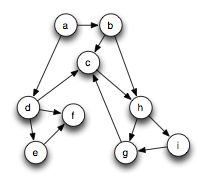
\includegraphics[width=0.25\textwidth]{aux/grafo}
	\caption[Estructura de un Grafo]{
	(tomada de \cite{BoostGrafos})}
	%\label{F-dimensions-emotion}
\end{figure}


\begin{figure}[H]
	\centering
	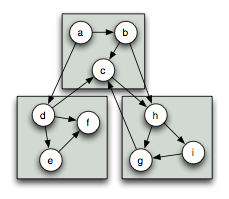
\includegraphics[width=0.25\textwidth]{aux/distributed-graph}
	\caption[Grafo Distribuido]{
	(tomada de \cite{BoostGrafos})}
	%\label{F-dimensions-emotion}
\end{figure}


\begin{figure}[H]
	\centering
	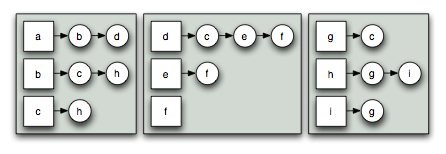
\includegraphics[width=0.5\textwidth]{aux/dist-adjlist}
	\caption[Grafo en lista de adyacencia]{
	(tomada de \cite{BoostGrafos})}
	%\label{F-dimensions-emotion}
\end{figure}


\begin{figure}[H]
	\centering
	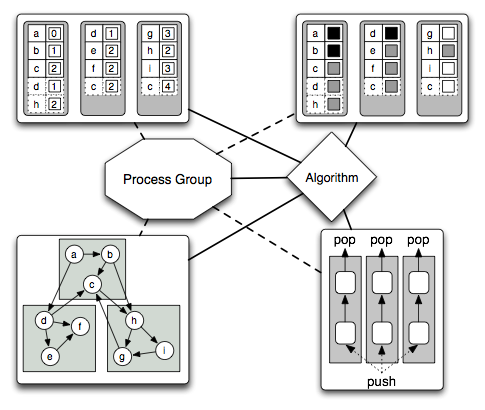
\includegraphics[width=0.5\textwidth]{aux/arquitectura_grafos}
	\caption[Aquitectura de Grafos]{
	(tomada de \cite{BoostGrafos})}
	%\label{F-dimensions-emotion}
\end{figure}


\section{C++}

C++ es un lenguaje de programación de propósitos generales,  que soporta abstracción de datos, es multiparadigma (programación estructurada, programación genérica\cite{andrei2001modern} y programación orientada a objetos).

C++ fue la elegido para este proyecto por su buen uso de los recursos computacionales, ampliamente reconocido como un lenguaje altamente eficiente, muy veloz y potente. \cite{stroustrup2013c++}


\section{MPI}

MPI es una interfaz de paso de mensajes individuales, ya sea punto a punto o de manera coordinada como grupo diseñado para permitir la comunicación entre varias unidades de computo, este surgió como un mecanismo para resolver la necesidad de permitir que múltiples procesos en paralelo trabajen de manera concurrente hacia la solución de un problema en particular. A diferencia de la comunicación en sistemas multihilos o de memoria compartida, MPI puede interactuar con diferentes sistemas operativos y arquitecturas subyacentes.   \cite{Karniadakis} \cite{BoostMPI}


\section{Boost}

Boost son una serie de librerías de C++, implementadas y mejoradas por la comunidad cuya base es el buen funcionamiento con la Librería Estandar de C++ (C++ STL) y la eventual estandarización de las mismas, mediante el mejoramiento progresivo de estas.\cite{wwwBoost}

Boost dentro de sus librerías tiene implementaciónes de programación genérica para grafos y adicionalmente una librería de algoritmos paralelos para grafos. \cite{siek2001boost}


\section{Parallel Boost Graph Library}

La PBGL es una librería de Boost para Grafos de Boost para computación paralela y distribuida. Esta ofrece algoritmos para computación en paralelo y distribuida, conservando las mismas interfaces que la librería secuencia para grafos de Boost.\cite{wwwBoost} 
